% ============================================================
% 分片：s02-duality  对应原文 PDF 第 13--21 页（印刷页 13--21）
% 负责章节：§2 Duality, Branes, and Endoscopy + 2.1--2.3（§2 标题起）
% 译者：trans-s02   审校状态：初稿
% ============================================================

% ==== 原文 PDF 第 13 页（印刷页 13）====

\section{对偶、膜与内窥}

\begin{keytakeaway}
\textbf{核心物理图像：}几何 Langlands 对应就是 Hitchin 纤维化的镜像对称：B-模型一侧取 $\mathcal{M}_H(C;{}^{L}G)$，其关于复结构 $J$ 的参数化给出 ${}^{L}G$-局部系统的模空间；A-模型一侧取 $\mathcal{M}_H(C;G)$，其关于复结构 $I$ 全纯的 Hitchin 纤维是特殊拉格朗日环面，逐纤维的 T-对偶把 B-膜映为 A-膜。当 ${}^{L}G$-局部系统的自同构群为有限群 $\Gamma$ 时，B-模型一侧的模空间出现轨形奇点，支撑于该点的 B-膜范畴成为 $\Gamma$ 的表示范畴；对偶地，A-模型一侧的奇异 Hitchin 纤维分裂为若干分支，$\Gamma$ 的每个不可约表示所对应的分数膜分别映到支撑在各分支上的不可约 A-膜。
\textbf{数学工具：}Hitchin 方程与超凯勒结构（复结构 $I,J,K$，实辛形式 $\omega_I,\omega_J,\omega_K$，全纯辛形式 $\Omega_I,\Omega_J,\Omega_K$）、Hitchin 纤维化与特征多项式、SYZ 特殊拉格朗日纤维化、$\mathcal{M}_H$ 的 Zariski 开集与 $T^*\mathcal{M}$ 的仿射辛形变、典范余迷向膜 $\mathcal{A}_{cc}$、扭 D-模与 $\mathcal{D}^*(\mathcal{L})$、本征膜与 Hecke 本征层。
\textbf{主要结论：}镜面对偶把 $\mathcal{M}_H(C;{}^{L}G)$ 上带有限自同构群 $\Gamma$ 的局部系统所对应的 B-膜分解（正则表示分解为 $\Gamma$ 的不可约表示），翻译为 $\mathcal{M}_H(C;G)$ 的奇异 Hitchin 纤维按同一组不可约表示分裂所给出的 A-膜分解；在 $G=SL_2$、${}^{L}G=SO_3$ 的情形，$A_1$ 奇点处的两个分数膜对应奇异纤维的两个分支，而相应的扭 D-模则分裂并满足分数 Hecke 本征层性质。
\end{keytakeaway}

\subsection{几何 Langlands 对偶与镜像对称}

在规范场论进路中，几何 Langlands 对应被理解为一种镜像对称。设 $\mathcal{Y}(C;G)$ 是定向二维流形 $C$ 上平坦 $G$-丛的模空间。\footnote{除另有说明外，总是指 Lie 群的复形式。这与几何 Langlands 纲领的多数文献一致，但与包括 [KW, GW] 在内的规范场论多数文献相反。}这里 $G$ 是复约化 Lie 群。于是 $\mathcal{Y}(C;G)$ 自然地是一个复辛流形。$\mathcal{Y}(C;G)$ 的复结构直接来自 $G$ 的复结构，其全纯二形式 $\Omega$ 则由 $\mathcal{Y}(C;G)$ 的切空间上的相交配对定义，而该切空间是 $H^1(C,\mathrm{ad}(Y))$。
% [原文疑误: 原文作 $H^1(C,\mathrm{ad}(Y))$，其中 $Y$ 与模空间 $\mathcal{Y}(C;G)$ 的记号撞名；按上下文应为某个局部系统（或平坦丛）的伴随丛，通常记作 $\mathrm{ad}(\mathcal{E})$。译文照录原文。 来源：原书 p.13 英文原文与译本对照（A）。]

利用 $\mathcal{Y}(C;G)$ 的复结构（以及其典范丛的平凡性，后者由 $\mathcal{Y}(C;G)$ 是复辛流形这一事实推出），可以定义 $\mathcal{Y}(C;G)$ 的 B-模型。类似地，把 $\mathcal{Y}(C;G)$ 视为实辛流形，其辛结构为 $\omega=\operatorname{Im}\Omega$，则可定义 A-模型。\footnote{$\Omega$ 的定义使得 $\operatorname{Im}\Omega$ 在上同调意义下平凡，而 $\operatorname{Re}\Omega$ 则不然。$\Omega$ 的定义依赖于 $\mathfrak{g}$（即 $G$ 的 Lie 代数）上一个非退化二次型的选择。然而，A-模型以及由此导出的几何 Langlands 对偶与这一选择无关，只差一个自然同构。一旦把平坦丛与 Higgs 丛之间的关系 [Hi1] 纳入，这一点便由 $\mathbb{C}^{*}$ 在 Higgs 丛模空间上的作用推出。在规范场论进路 [KW] 中，先验地清楚这一选择无关紧要，因为作用量对规范耦合的依赖具有 $\{Q,\cdot\}$ 的形式。}

现在设 ${}^{L}G$ 与 $G$ 是一对互为对偶的复约化 Lie 群。结果表明，$\mathcal{Y}(C;{}^{L}G)$ 的 B-模型与 $\mathcal{Y}(C;G)$ 的 A-模型之间存在镜像对称。这一实例的镜像对称最早由 Hausel 与 Thaddeus [HT] 研究。（接近的对偶性已由 Donagi 与 Pantev [DP]、Hitchin [Hi3] 以及 Arinkin [Ari] 研究过；二者之间的关系在第 5.3 节说明。）它是从四维超对称规范场论的电-磁对偶推出的 [KW]，其依据是更早的论证 [BJSV, HMS]，并被证明构成几何 Langlands 对偶的基础。\footnote{我们将把自己限制在几何 Langlands 对偶最基本的形式上。在 [KW] 中解释了如何在规范场论进路中纳入一个额外的复参数，从而导致数学文献中有时所谓的量子几何 Langlands。}

% ==== 原文 PDF 第 14 页（印刷页 14）====

为了建立 $\mathcal{Y}(C;{}^{L}G)$ 与 $\mathcal{Y}(C;G)$ 之间的镜像对称，需要如下事实：这两个空间还有另一种解释，即作为 Higgs 丛的模空间。这来自 Hitchin 方程。与我们此前考虑的 $\mathcal{Y}(C;G)$ 的复辛结构不同，Hitchin 方程要求对 $C$ 的共形结构作一选择。因此从现在起，$C$ 是复 Riemann 面，而不只是一个定向二维流形。

\subsubsection{Hitchin 方程}

Hitchin 方程 [Hi1] 是关于一对 $(A,\phi)$ 的非线性方程。$A$ 是 $G$-丛 $E\to C$ 上的一个联络，该丛的结构群为 $G$ 的紧实形式；而 $\phi$ 是 $C$ 上取值于 $\mathfrak{g}$（即该紧实形式的 Lie 代数）的一形式。Hitchin 方程写作
\begin{equation}\tag{2.1}
\begin{aligned}
F - \phi\wedge\phi &= 0\\
d_A\phi = d_A\star\phi &= 0.
\end{aligned}
\end{equation}
这里 $d_A$ 是规范协变外微分，$\star$ 是 Hodge 星算子。

若 $(A,\phi)$ 是 Hitchin 方程的解，则 $\mathcal{A}=A+\ii\phi$ 是复值平坦联络，从而赋予 $E$（或其复化）以局部系统的结构。特别地，Hitchin 方程的一个解确定了 $\mathcal{Y}(C;G)$ 中的一个点，即结构群为 $G$ 的局部系统的模空间中的一点。
% [Tutor Note: 跳步点拨。由 (2.1) 到「$\mathcal{A}=A+\ii\phi$ 平坦」只需直算：$\mathcal{A}$ 的曲率为 $F_{\mathcal{A}}=F_A+\ii d_A\phi-\phi\wedge\phi$，其实部为 $F_A-\phi\wedge\phi$、虚部为 $d_A\phi$。另注意在二维基流形上 Hodge 星算子把一形式仍映为一形式，故 $d_A\star\phi=\pm\star d_A\phi$，于是 (2.1) 第二行的两个等式彼此等价，Hitchin 方程实质上就是「$F_A=\phi\wedge\phi$ 且 $d_A\phi=0$」。 来源：原书 p.14 上下文（A）。]

另一种看法是：由算子 $d_A$ 的 $(0,1)$ 部分给出的 $\bar\partial$ 算子赋予 $E$ 以全纯结构。若把 $\phi$ 的 $(1,0)$ 部分记作 $\varphi$、把 $C$ 的典范丛记作 $K$，则 $\varphi$ 是 $K\otimes\mathrm{ad}(E)$ 的截面，并且按 Hitchin 方程它是全纯的。于是对 $(E,\varphi)$ 定义了从全纯观点看所谓的 Higgs 丛。

关于 Hitchin 方程的一个基本结果是：这些方程的解的模空间 $\mathcal{M}_H=\mathcal{M}_H(C;G)$ 是超凯勒流形。在一个复结构下（[Hi1] 中称之为 $I$），$\mathcal{M}_H$ 是稳定 Higgs 丛的模空间；而在另一个复结构下（记作 $J$），它是稳定局部系统的模空间，并且与我们此前称为 $\mathcal{Y}$ 的空间一致。同一个空间具有这两种对偶解释，正是在研究 Higgs 丛时能够对几何 Langlands 说些什么的原因之一。

作为超凯勒流形，$\mathcal{M}_H$ 具有一个特殊的实辛形式三元组 $\omega_I,\omega_J,\omega_K$，它们分别在复结构 $I$、$J$ 与 $K=IJ$ 下是 Kähler 形式。类似地，有复二形式 $\Omega_I=\omega_J+\ii\omega_K$、$\Omega_J=\omega_K+\ii\omega_I$、$\Omega_K=\omega_I+\ii\omega_J$，它们分别在复结构 $I$、$J$ 与 $K$ 下是全纯辛形式。当 $\mathcal{Y}$ 与 $\mathcal{M}_H$ 等同起来时，其复结构对应于 $J$；此外，其全纯辛形式为 $\Omega=\ii\Omega_J$，而 $\omega=\operatorname{Im}\Omega$ 等于 $\omega_K$。
% [Tutor Note: 易错预警。这里有三处约定必须核对：(i) A-模型用的辛形式是 $\omega=\operatorname{Im}\Omega=\omega_K$，而非 $\operatorname{Re}\Omega$；(ii) 复结构 $K=IJ$ 是 $I$ 与 $J$ 的复合，方向不同会改变 $\Omega_K$ 的符号；(iii) $\Omega_I=\omega_J+\ii\omega_K$ 中的虚数单位在本译本中按 GLOSSARY 统一排作直立体 $\mathrm{i}$，原书排作斜体 $i$。另注意 $(E,\varphi)$ 中的 Higgs 场在全文中记作 $\varphi$，而 Hitchin 方程中取值于 $\mathfrak{g}$ 的一形式记作 $\phi$，二者不可混用。 来源：原书 p.14 上下文（A）。]

\subsubsection{Hitchin 纤维化}

Hitchin 纤维化是把 Higgs 丛 $(E,\varphi)$ 映到 $\varphi$ 的特征多项式的映射 $\Pi:\mathcal{M}_H\to\boldsymbol{B}$。（$\boldsymbol{B}$ 是参数化特征多项式一切可能取值的线性空间。）

% ==== 原文 PDF 第 15 页（印刷页 15）====

Hitchin 纤维化在复结构 $I$ 下全纯（在复结构 $I$ 下 $\mathcal{M}_H$ 是 Higgs 丛的模空间）。从全纯辛结构 $\Omega_I$ 的观点看，该纤维化的纤维是拉格朗日子流形，从而从 $\omega_K=\operatorname{Im}\Omega_I$ 的观点看也是如此。

于是，从几何 Langlands 纲领中所涉及的 A-模型的观点看，Hitchin 纤维化是一个由拉格朗日子流形构成的纤维化。这些纤维一般地是光滑环面（关于复结构 $I$ 全纯）。这一事实与把 $\mathcal{M}_H$ 解释为完全可积 Hamilton 系统 [Hi2] 有关，并且可用谱曲线显式看出，正如我们将在第 5 节解释的那样。
% [Tutor Note: 物理图像。$\Pi$ 关于 $I$ 全纯而 $\Omega_I$ 关于 $I$ 全纯辛，故纤维是复拉格朗日子流形，其复维数为 $\tfrac12\dim_{\mathbb{C}}\mathcal{M}_H$；又因 $\omega_K=\operatorname{Im}\Omega_I$ 限制到纤维上为零，纤维同时是 $(\mathcal{M}_H,\omega_K)$ 的实拉格朗日子流形。一般纤维是阿贝尔簇（对 $SL_n$ 为谱曲线的 Prym 簇），这正是「完全可积」的含义：$\Pi$ 的纤维是 Lagrangian 环面，其上的平移给出可积系统的直线流。 来源：原书 p.15 上下文（A）。]

从 A-模型的观点看，Hitchin 纤维化的纤维不只是拉格朗日环面，它们是特殊拉格朗日的。事实上，由于它们关于诸复结构之一（即 $I$）全纯，它们在自己的上同调类中极小化体积（用 $\mathcal{M}_H$ 的超凯勒度量计算）。因此 [HT] 这是由特殊拉格朗日环面构成的纤维化的一个例子，而这种几何结构被提出 [SYZ] 用来描述镜像对称。
% [Tutor Note: 推导补足。「关于某个复结构全纯的拉格朗日子流形是特殊拉格朗日的」是超凯勒几何中的标准事实：若 $L$ 关于 $I$ 全纯且关于 $\omega_K=\operatorname{Im}\Omega_I$ 为拉格朗日，则由 $\Omega_I$ 关于 $I$ 是 $(2,0)$-形式可知 $\Omega_I|_L=\omega_J|_L$ 为实形式，即 $L$ 被校准形式 $\operatorname{Re}\Omega_I=\omega_J$ 校准，从而在其上同调类中极小化体积。原文把这一标准结论压成一句「因此它们在自己的上同调类中极小化体积」，此即 SYZ 图景所需的特殊拉格朗日条件。 来源：原书 p.15 上下文（A）。]

更具体地说，若 $G$ 是单链（simply-laced）的，则 $G$ 与 ${}^{L}G$ 的 Hitchin 纤维化的底相同。（例如在第 3 节中，我们将对 $G=SL_2$ 与 ${}^{L}G=SO_3$ 用同一个复变量 $w$ 来参数化 $\boldsymbol{B}$。）对任何 $G$，这些底之间都有自然同构。于是我们得到一幅图景：
\begin{equation}\tag{2.2}
\begin{array}{ccccc}
\mathcal{M}_H({}^{L}G) & & & & \mathcal{M}_H(G)\\[2pt]
& \searrow & & \swarrow & \\[2pt]
& & \boldsymbol{B} & &
\end{array}
\end{equation}
这两个纤维化在一般点 $b\in\boldsymbol{B}$ 上的纤维是对偶环面，这一点最早在 [HT] 中对 $G=SL_n$ 论证过。（对其它群见 [DP, Hi3]。）这就是与镜像对称相联系的通常的 SYZ 图景。

这一特别的例子有几个优点。具体描述一个特殊拉格朗日纤维化通常极为困难，但在 $\mathcal{M}_H$ 的情形，纤维化关于复结构 $I$ 全纯这一事实使它成为可及的，正如我们将在第 3 节与第 5.3 节所讨论的例子中看到的那样。此外，镜像对称与特殊拉格朗日纤维化之间的关系通常会受到物理学家所谓盘瞬子（disc instanton）量子修正的影响。然而，$\mathcal{M}_H$ 的超凯勒性质保证这类修正不存在，从而使 Hitchin 纤维化在镜像对称的这一特别例子中的应用更为直接。

\subsection{膜及其对偶}

为了与几何 Langlands 对偶建立联系，我们必须考虑 $\mathcal{M}_H$ 上的 B-膜与 A-膜。

一个简单的 B-膜 $\mathcal{B}$ 的例子，是支撑在光滑点 $r\in\mathcal{M}_H(C;{}^{L}G)$ 上的秩 1 膜。这样的点对应于 $C$ 上的一个不可约 ${}^{L}G$ 局部系统 $\mathcal{E}_r$（即自同构群收缩到 ${}^{L}G$ 的中心者；暂且假设该中心平凡）。它包含在 ${}^{L}G$ 的 Hitchin 纤维化的纤维 ${}^{L}\boldsymbol{F}_b$ 中，并位于该纤维化的底 $\boldsymbol{B}$ 中的点 $b$ 之上。我们以 $\boldsymbol{F}_b$ 记 $\mathcal{M}_H(C;G)$ 的对偶 Hitchin 纤维化在 $b$ 上的纤维。

% ==== 原文 PDF 第 16 页（印刷页 16）====

镜像对称被理解为 Hitchin 纤维化纤维上的 T-对偶。于是它把 $\mathcal{B}$ 映到支撑为 $\boldsymbol{F}_b$ 的 A-膜 $\mathcal{A}$，并带有依赖于 $r$ 的平坦酉线丛 $\mathcal{L}_r$。这是合理的，因为对偶 Hitchin 纤维化的一般纤维 ${}^{L}\boldsymbol{F}_b$ 与 $\boldsymbol{F}_b$ 是对偶环面。因此点 $r\in{}^{L}\boldsymbol{F}_b$ 确定一个平坦酉线丛 $\mathcal{L}_r\to\boldsymbol{F}_b$。

上面描述的只是通常的图景。若 $r$ 是 $\mathcal{M}_H(C;{}^{L}G)$ 中的奇异点，即对应于一个具有非平凡自同构群的 ${}^{L}G$ 局部系统，情形又如何？支撑在光滑点上的膜范畴等价于向量空间范畴，其等价由把膜映到其截面空间的映射给出。支撑在奇异点上的膜范畴一般更为复杂，不能约化为单个对象。镜像对称或几何 Langlands 对偶必须应用于这整个范畴。
% [Tutor Note: 易错预警。「点上的膜范畴 $\simeq$ 向量空间范畴」只在点是光滑点时成立：此时结构层可分裂地取定，任意膜是某个向量空间与点层的直和，膜之间的态射就是线性映射。奇异点处模空间局部为 $\mathbb{C}^{2n}/\Gamma$，膜范畴变成 $\Gamma$-等变（或 $\Gamma$-分次）向量空间范畴，不能由单个对象生成，故原文强调对偶必须作用于整个范畴而不仅是某个对象。 来源：原书 p.16 上下文（A）。]

现在假设局部系统 $\mathcal{E}_r$ 的自同构群是非平凡有限群 $\Gamma$。此时 ${}^{L}G$ 局部系统的模空间在 $r$ 附近可以建模为有限商 $\mathbb{C}^{2n}/\Gamma$（对某个 $n$），其中 $\Gamma$ 在 $\mathbb{C}^{2n}$ 上的线性作用来自同态 $\Gamma\to Sp_{2n}\subset U_{2n}$。（$\Gamma$ 通过辛群的子群作用，因为 $\mathcal{M}_H$ 是复辛的，事实上是超凯勒的。）我们把 $r$ 等同于 $\mathbb{C}^{2n}/\Gamma$ 的原点。支撑在 $r$ 上的膜的截面空间现在是带 $\Gamma$ 作用的有限维向量空间。要描述一个膜，我们必须说明 $\Gamma$ 如何作用在这个向量空间上。不可约膜对应于不可约表示。（更完整的描述见第 10 节。）

即使 $\Gamma$ 就是 ${}^{L}G$ 的中心，使用这套形式体系也是有意义的；此时 $r$ 是光滑点，因为中心在进入 Hitchin 方程的场上平凡地作用。中心的一个不可约表示是一维的，由 [KW] 第 7 节中称为 $\boldsymbol{e}_0$ 的特征标给出。于是，光滑点处不可约膜的描述可以细化为同时指定特征标 $\boldsymbol{e}_0$。在对偶之下，$\boldsymbol{e}_0$ 映为特征类 $\boldsymbol{m}_0\in H^2(C,G)$，它决定了 $C$ 上 $G$-丛的拓扑。$\mathcal{M}_H(C;{}^{L}G)$ 上指定了 $\boldsymbol{e}_0$ 的膜，其对偶支撑在 $\mathcal{M}_H(C;G)$ 中具有确定 $\boldsymbol{m}_0$ 的不可约分支上。
% [Tutor Note: 推导补足。$\boldsymbol{e}_0$ 是中心 $Z({}^{L}G)$ 的特征标，在 [KW] 的规范场论语言中即「离散电参数」；对偶之下它成为 $G$-丛的「离散磁参数」，即决定 $G$-丛在 $\Bun_G$ 中所在连通分支的拓扑类（'t Hooft 磁通）。原文把这一对应记为 $\boldsymbol{e}_0\mapsto\boldsymbol{m}_0$，本质上是中心对偶 $Z({}^{L}G)^{\wedge}\cong Z(G)$ 在丛拓扑上的几何表现；中心平凡时两侧均退化，故下文转入内窥。 来源：原书 p.16 上下文（A）。]

然而，内窥出现在自同构群不只是中心的时候；我们将假设 ${}^{L}G$ 的中心平凡来说明这些想法。例如在第 3 节的例子中，我们将取 ${}^{L}G=SO_3$，其中心平凡。这样一来，$\Gamma$ 有效地作用在 $\mathbb{C}^{2n}$ 上；若 $\Gamma$ 非平凡，则 $r$ 是 $\mathcal{M}_H(C;{}^{L}G)$ 的轨形奇点。此时，对 $\Gamma$ 的每个不可约表示 $R_i$ 的同构类，都有相应的不可约膜 $\mathcal{B}_i$ 支撑在点 $r$ 上。

设 $r^*$ 是 $\mathcal{M}_H(C;{}^{L}G)$ 的光滑点，带有不可约膜 $\mathcal{B}^*$。现在考虑当 $r^*$ 逼近轨形点 $r$ 时会发生什么。在极限下，不可约膜 $\mathcal{B}^*$ 退化为支撑在 $r$ 上、与 $\Gamma$ 的正则表示相联系的膜。（其原因在于：光滑点 $r^*\in\mathbb{C}^{2n}/\Gamma$ 对应于 $\mathbb{C}^{2n}$ 上的一个自由 $\Gamma$-轨道；自由轨道上的函数提供正则表示的一份拷贝。）正则表示可以分解为 $\bigoplus_i n_iR_i$，其中求和遍历 $\Gamma$ 的所有不可约表示 $R_i$，$n_i$ 是 $R_i$ 的维数。于是 $\mathcal{B}^*$ 的分解为
\begin{equation}\tag{2.3}
\mathcal{B}^*\to\bigoplus_i n_i\mathcal{B}_i.
\end{equation}

% ==== 原文 PDF 第 17 页（印刷页 17）====

在物理学文献中，这一分解最早在 [DM] 中分析过，而膜 $\mathcal{B}_i$ 通常称为\emph{分数膜}（fractional branes）。
% [Tutor Note: 推导补足。「膜在极限下退化为正则表示」的准确含义是：$\mathbb{C}^{2n}/\Gamma$ 上的一个自由轨道在极限下坍缩为原点，其上的函数空间（正则表示）在推前（取 $\Gamma$-不变量）后分解为各不可约表示，重数为维数 $n_i=\dim R_i$。这正是 McKay 对应在膜范畴层面的表现：轨形点上的不可约膜与 $\Gamma$ 的不可约表示一一对应，而光滑点的点膜退化为这些不可约膜的直和。 来源：原书 p.17 上下文（A）。]

这一分解对镜像对称或几何 Langlands 对偶意味着什么？对光滑点 $r^*$，膜 $\mathcal{B}^*$ 是不可约的，并被对偶映到支撑在 $G$ 的 Hitchin 纤维化的相应纤维 $\boldsymbol{F}^*$ 上的 A-膜 $\mathcal{A}^*$。$\boldsymbol{F}^*$ 作为拉格朗日子流形是不可约的，所以相应的膜作为 A-膜也是不可约的。当把 $r^*$ 取为 $r$ 时，膜 $\mathcal{B}^*$ 分解为若干 B-膜之和，因此对偶的 A-膜 $\mathcal{A}^*$ 也必须分解为若干 A-膜之和，
\begin{equation}\tag{2.4}
\mathcal{A}^*\to\bigoplus_i n_i\mathcal{A}_i.
\end{equation}
这一分解若能几何地发生，将是很有吸引力的。（事实上，我们不知道它还可能以其它方式发生。）在第 3 节与第 5 节中，我们将对 ${}^{L}G=SO_3$ 详细说明几何分解如何发生。在这个例子中，$\mathcal{M}_H(C;{}^{L}G)$ 含 $A_1$ 奇点，对应于自同构群为 $\mathbb{Z}_2$ 的局部系统。（这些是内窥局部系统的最简单例子。）设 $r$ 是这些奇点之一。同构意义下，支撑在 $r$ 上的不可约膜有两个，记为 $\mathcal{B}_+$ 与 $\mathcal{B}_-$，分别对应于 $\mathbb{Z}_2$ 的两个一维表示，其中非平凡元素分别作用为 $+1$ 或 $-1$。分解 (2.3) 读作
\begin{equation}\tag{2.5}
\mathcal{B}^*\to\mathcal{B}_+\oplus\mathcal{B}_-.
\end{equation}
相应地，$G=SL_2$ 的相应 Hitchin 纤维应当分解为两个分支之和。

我们将在第 3 节对 $G=SL_2$ 的亏格一情形、在第 5 节的高亏格情形中显式看到这一点。恰在 Hitchin 纤维化的底 $\boldsymbol{B}$ 中那些使 ${}^{L}G=SO_3$ 的模空间含有奇点的点之上，$G=SL_2$ 的 Hitchin 纤维化的纤维分解为两个分支 $\boldsymbol{F}_1$ 与 $\boldsymbol{F}_2$ 的并，二者在两个二重点处相交。在第 3 节所研究的例子（亏格一、一个分歧点）中，$\boldsymbol{F}_1$ 与 $\boldsymbol{F}_2$ 都同构于 $\mathbb{C}\mathbb{P}^1$。它们光滑，且光滑地嵌入 $\mathcal{M}_H(C;G)$，各自本身都是 A-膜。我们的提议是：支撑在轨形奇点 $r\in\mathcal{M}_H(C;{}^{L}G)$ 上的两个分数膜 $\mathcal{B}_+$ 与 $\mathcal{B}_-$ 在对偶下分别映到支撑在 $\boldsymbol{F}_1$ 与 $\boldsymbol{F}_2$ 上的 A-膜 $\mathcal{A}_1$ 与 $\mathcal{A}_2$。（$\mathcal{B}_+$ 与 $\mathcal{B}_-$ 中哪一个映到 $\mathcal{A}_1$、哪一个映到 $\mathcal{A}_2$，是一个略为微妙的问题，将在第 10 节讨论。）

% ==== 原文 PDF 第 18 页（印刷页 18）====

\begin{figure}[H]
\centering
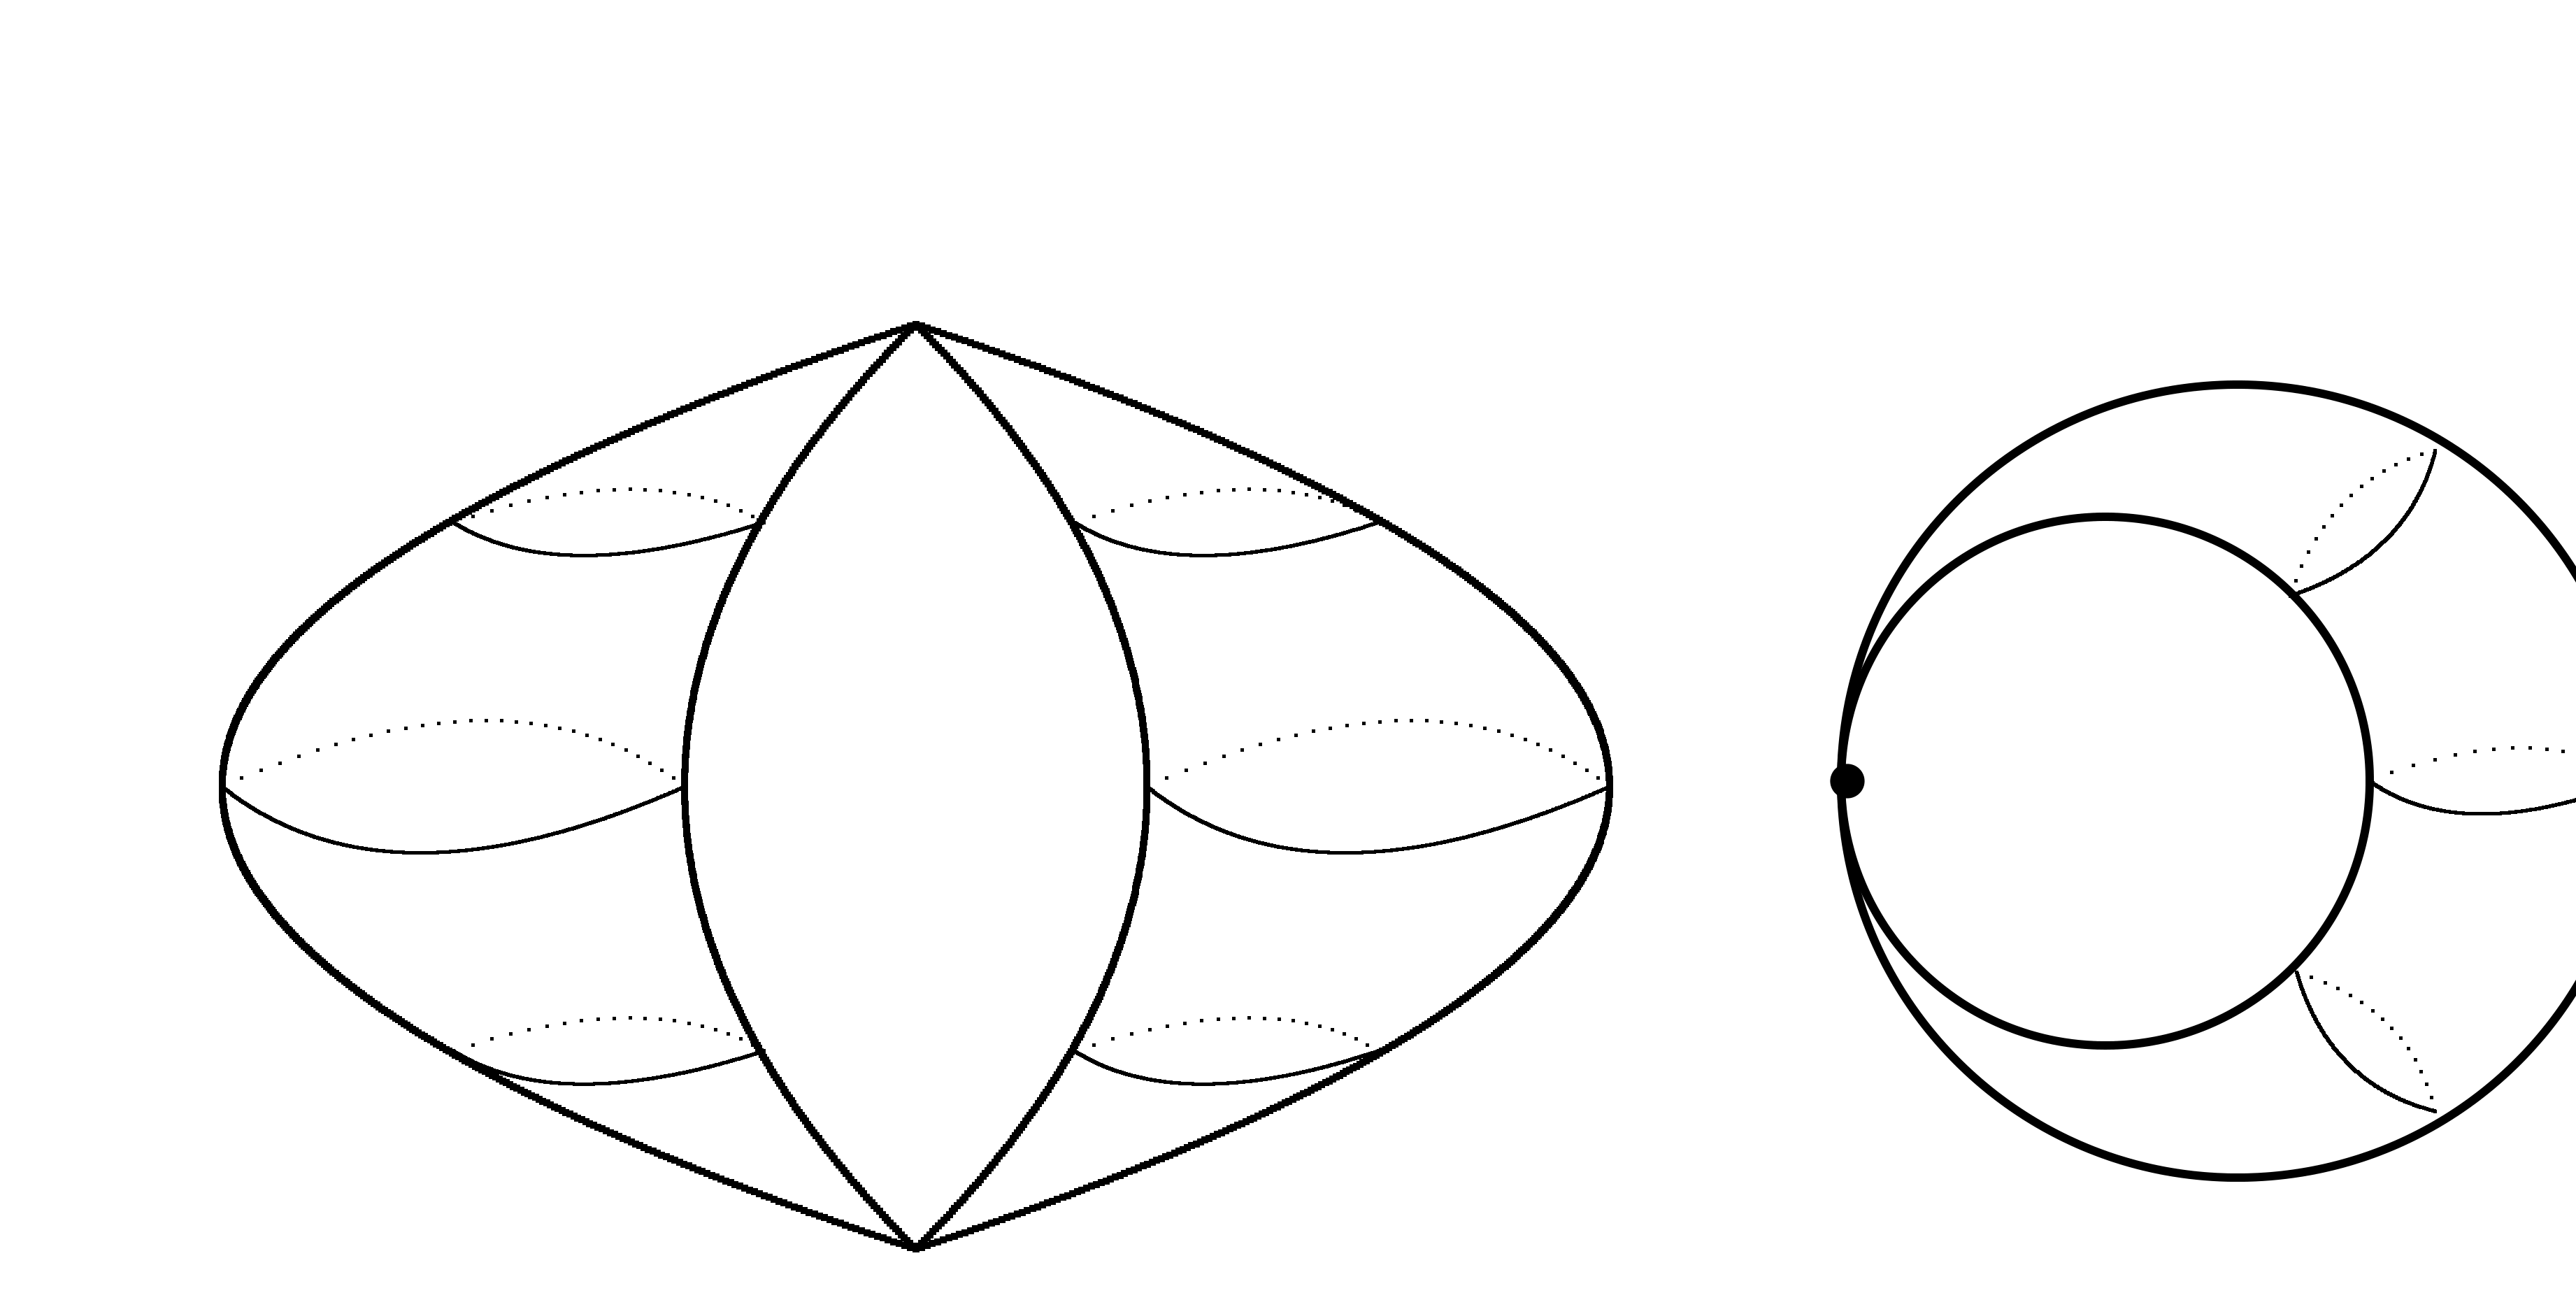
\includegraphics[width=0.92\textwidth]{figures/fig-p18-hitchin-fibers.png}
\caption{奇异 Hitchin 纤维。左：$A$-模型一侧，$G=SL_2$；右：$B$-模型一侧，${}^{L}G=SO_3$。（原书 p.18；原图无编号）}
\label{fig:p18-hitchin-fibers}
\end{figure}

尽管本文的细致分析将限于 ${}^{L}G=SO_3$、$G=SL_2$，我们的猜想是：对内窥的类似几何描述对所有群都成立（见第 9 节）。

\subsection{从 A-膜到 D-模}

至此所讨论的是 $\mathcal{M}_H(C;G)$ 上与 $\mathcal{M}_H(C;{}^{L}G)$ 上的 B-膜相对偶的 A-膜。然而，B-膜的几何 Langlands 对偶通常不是描述为 A-膜，而是描述为曲线 $C$ 上稳定 $G$-丛的模空间 $\mathcal{M}$（更一般地说，$C$ 上 $G$-丛的模叠 $\Bun_G$）上的扭 D-模。
% [Tutor Note: 易错预警。这里同时出现三个「模空间」：$\mathcal{M}_H$（Hitchin 模空间，超凯勒）、$\mathcal{M}$（稳定 $G$-丛的模空间，即 $\Bun_G$ 的稳定部分）、$T^*\mathcal{M}$（其余切丛）。原文用 $\mathcal{M}$ 而非 $\mathcal{M}_H$ 指后者，切勿与 Higgs 丛模空间混淆；$\mathcal{M}_H$ 只在非分歧情形才等于 $T^*\mathcal{M}$，有分歧时须换成仿射辛形变（见第 3.9 节）。 来源：原书 p.18 上下文（A）。]

这两种观点在 [KW] 第 11 节中得到调和。最熟悉的 A-膜是支撑在拉格朗日子流形（例如 Hitchin 纤维化的纤维）上、并带有平坦酉联络的膜。然而，辛流形 $X$ 上的 A-模型一般 [KO] 还可以有额外的膜，它们支撑在维数可能超过 $X$ 的一半维数的余迷向子流形上。特别地，设 $X=T^*Y$ 是复流形 $Y$ 的余切丛，带有自然的全纯二形式 $\Omega$。考虑 $X$ 上以辛形式 $\omega=\operatorname{Im}\Omega$ 定义的 A-模型。该 A-模型容许一个特殊的膜，即典范余迷向 A-膜 $\mathcal{A}_{cc}$，其支撑是整个 $X$，其存在弥合了 A-膜与 D-模之间的鸿沟。$\mathcal{A}_{cc}$ 的自同态（用物理术语说，即 $\mathcal{A}_{cc}-\mathcal{A}_{cc}$ 弦）可以沿 $Y$ 层化，给出一个环层。这个环层就是作用在 $K_Y^{1/2}$ 上的微分算子层，其中 $K_Y$ 是 $Y$ 的典范丛。我们以 $\mathcal{D}^*$ 记这样的微分算子层，并把此环层上的模层（或下文引入的其推广）称为扭 D-模。现在，若 $\mathcal{A}$ 是任何其它 A-膜，则 $\operatorname{Hom}(\mathcal{A}_{cc},\mathcal{A})$ 可以沿 $\mathcal{M}$ 层化，给出一个扭

% ==== 原文 PDF 第 19 页（印刷页 19）====

D-模。对应 $\mathcal{A}\to\operatorname{Hom}(\mathcal{A}_{cc},\mathcal{A})$ 给出一个从 A-膜范畴到扭 D-模范畴的函子。
% [Tutor Note: 推导补足。为什么自同态层给出「作用在 $K_Y^{1/2}$ 上的微分算子」？因为 $\mathcal{A}_{cc}$ 的支撑是整个 $X$，其开弦态空间在 $T^*Y$ 上局部由多项式函数（沿纤维方向）张成，沿 $Y$ 层化后得到 Weyl 代数层；再对 $Y\subset T^*Y$ 的横截方向作半无限形式的量子化（或等价地取 Weyl 代数的中心化子），即得作用在 $K_Y^{1/2}$ 上的微分算子层。$K_Y^{1/2}$ 的出现是半密度/半形式的必然结果，也是整篇「A-膜到 D-模」对应中唯一依赖 $Y$ 的几何信息之处。 来源：原书 p.19 上下文（A）。]

要把这一点应用到 $\mathcal{M}_H$ 上的 A-膜，我们注意到：虽然 $\mathcal{M}_H$ 并不恰好是余切丛，它含有一个可与 $T^*\mathcal{M}$ 等同的 Zariski 开集，其中 $\mathcal{M}$ 是稳定丛的模空间。$\mathcal{M}_H$ 上的 A-膜 $\mathcal{A}$ 可以限制到 $T^*\mathcal{M}$，而且由于维数理由这一限制非空。于是可以应用上述构造，把 $\mathcal{A}$ 联系到 $\mathcal{M}$ 上的扭 D-模。
% [Tutor Note: 易错预警。「由于维数理由限制非空」指的是：$\mathcal{A}$ 的支撑是实维数 $\ge\dim_{\mathbb{R}}\mathcal{M}_H$ 的余迷向子流形（拉格朗日膜恰为一半维数），而 $\mathcal{M}_H\setminus T^*\mathcal{M}$ 的余维为正，故支撑必与 $T^*\mathcal{M}$ 相交。这一步在原文中被一笔带过，但它是「A-膜总能给出 D-模」的关键；若支撑整个落在例外除子上，构造就会失效，而这里不会发生。 来源：原书 p.19 上下文（A）。]

这一构造有一个类比，其中 $X$ 不是 $Y$ 的余切丛，而是它的仿射辛形变。这意味着 $X\to Y$ 是仿射空间的丛，带有全纯辛形式 $\Omega$，使得沿 $Y$ 局部地 $X$ 等价于 $T^*Y$。这样的 $X$ 可由 $T^*Y$ 经元素\footnote{为构造 $X$，把 $\chi$ 拉回到 $H^1(T^*Y,\Omega^{1,\mathrm{cl}}(T^*Y))$，并用 $T^*Y$ 的辛形式把这个拉回映到 $H^1(T^*Y,T(T^*Y))$，后者分类 $T^*Y$ 的形变。所得形变是辛的，因为我们从 $\Omega^{1,\mathrm{cl}}$ 出发。}$\chi\in H^1(Y,\Omega^{1,\mathrm{cl}})$ 扭转得到，其中 $\Omega^{1,\mathrm{cl}}$ 是 $Y$ 上闭一形式的层。在这种情形，仍然可以定义\footnote{需要要求 $\operatorname{Re}\chi$ 的上同调类等于 [GW] 中称为 $\eta$ 的量子参数。除第 4.7 节外，我们强调经典图景并略去 $\eta$ 的作用。}典范余迷向膜 $\mathcal{A}_{cc}$，而 $\mathcal{A}_{cc}$ 的自同态仍然可以沿 $Y$ 层化。此时所得的环层是作用在 $K_Y^{1/2}\otimes\mathcal{L}$ 上的微分算子层，其中\footnote{一般地，$\chi$ 的上同调类不是整的，所以 $\mathcal{L}$ 可能是线丛的复幂（或这种幂的张量积），而不是普通的复线丛。但作用在 $\mathcal{L}$ 上、或作用在 $K_Y^{1/2}\otimes\mathcal{L}$ 上的微分算子层仍然有意义。}$\mathcal{L}$ 是一个「线丛」，满足 $c_1(\mathcal{L})=\chi$。于是我们得到一个从 $Y$ 上 A-膜到 $\mathcal{D}^*(\mathcal{L})$ 的模的函子，其中 $\mathcal{D}^*(\mathcal{L})$ 是作用在 $K_Y^{1/2}\otimes\mathcal{L}$ 上的微分算子层。

这一构造在 [KW] 中被应用于数学上所谓的量子几何 Langlands。（这里需要考虑取复结构为对 $I$ 作超凯勒旋转所得复结构下的 $X=\mathcal{M}_H$。）与我们的目的更相关的是，它被 [GW] 应用于几何 Langlands 的分歧情形。这里用到的事实是：在分歧情形，$\mathcal{M}_H$ 中的一个 Zariski 开集可以等同于 $T^*\mathcal{M}$ 的一个仿射辛形变。（对本文的例子，这在第 3.9 节有详细描述。）对几何 Langlands 的分歧情形，这一构造导致如下陈述：存在一个从 $\mathcal{M}_H(C;G)$ 的 A-膜到 $\mathcal{M}$ 上 $\mathcal{D}^*(\mathcal{L})$-模的自然函子，其中 $\mathcal{M}$ 现在是 $C$ 上稳定抛物 $G$-丛的模空间，而 $\mathcal{L}$ 的第一陈类是对偶 ${}^{L}G$ 局部系统的单值的对数。

\subsubsection{与局部系统的关系}

现在讨论在此情形中由 A-膜产生的扭 D-模如何与局部系统相联系。设 $X$ 为 $T^*Y$ 或其一仿射形变，并设 $\pi:X\to Y$ 为投影。设 $L$ 是 $X$ 的一个紧（复）拉格朗日子流形，使得映射 $\pi:L\to Y$ 是 $n$ 重覆盖。那么从 A-膜到扭 D-模的函子预期把支撑在 $L$ 上的秩 1 A-膜映为 $Y$ 上秩 $n$ 的局部系统（被 $K_Y^{1/2}$ 扭），换言之，映为 $Y$ 上带有平坦联络（或在仿射形变情形带有中心曲率联络）的秩 $n$ 复向量丛 $V\to Y$。

% ==== 原文 PDF 第 20 页（印刷页 20）====

若 $L$ 在 $X$ 中闭而不紧，且映射 $\pi:L\to Y$ 一般地是 $n$ 对 1、但在一个除子上次数较低，则上述结论有一个重要的推广。这在直观上发生的情形是：$L$ 的某些分支在所论除子之上趋于无穷远。为简单起见，假设 $Y$ 是曲线，第 3 节的例子实际上就是这种情况。设 $u$ 是 $Y$ 上的局部参数，设 $s$ 是 $X\to Y$ 的纤维上的线性函数，使得沿 $Y$ 局部地 $X$ 的辛形式为 $\Omega=du\wedge ds$。则 $L$ 可以局部地由一个 $n$ 值函数 $s(u)$ 描述，而我们所关心的情形是这个函数的某些分支在点 $r\in Y$（对应于比如 $u=u_0$）处奇异。我们假设这 $n$ 个分支形如
\begin{equation}\tag{2.6}
s_i(u)\sim c_i(u-u_0)^{-d_i},\qquad i=1,\dots,n.
\end{equation}
（$d_i$ 不必是整数，因为映射 $\pi:L\to Y$ 可能在 $u=u_0$ 处分歧。）在这种情形，支撑在 $L$ 上的 A-膜将映为 $Y$ 上的扭 D-模，后者由在 $r$ 处带奇点的局部系统 $V\to Y\setminus\{r\}$ 表示。奇点的性质在很大程度上由 $d_i$ 与 $c_i$ 决定。例如，正则奇点的条件是 $d_i\le 1$，而正则奇点处的单值也在很大程度上由 $c_i$ 决定。由于这个原因，我们在式 (3.49) 中为本文的例子计算 $c_i$ 与 $d_i$。在第 4 节中，我们解释这些系数预期如何与局部系统的奇点相联系，并描述向高维的推广。
% [Tutor Note: 易错预警。(2.6) 中的 $d_i$ 与 $c_i$ 互为独立的资料：$c_i$ 决定正则奇点处的单值（即共振项，经 $\exp(2\pi\ii c_i)$ 型公式），$d_i$ 决定奇点的阶（正则 vs 不规则）。条件 $d_i\le1$ 只是正则性的必要条件，真正的正则性还要看 $d_i$ 为整数时的对数项；原文只给出必要条件并说明「在很大程度上决定」，阅读时不可把 $d_i\le1$ 当作充分条件。 来源：原书 p.20 上下文（A）。]

\subsubsection{本征膜与本征层}

$\mathcal{M}_H$ 的镜像对称具有许多与它源自四维理论有关的特殊性质。例如，四维规范场论的 Wilson 与 't Hooft 线算子可以在二维意义下重新解释 [KW]，它们对于理解几何 Langlands 纲领的 Hecke 算子至关重要。

从 A-膜到 D-模的对应应当把 't Hooft 算子的本征 A-膜映为 $\mathcal{M}$ 上的 D-模（更一般地，映为曲线 $C$ 上 $G$-丛的模叠 $\Bun_G$ 上的 D-模），后者是 Hecke 本征层。这些 Hecke 本征层是几何 Langlands 对应（在其通常表述中）所关注的主要对象。几何 Langlands 猜想预言：对 $C$ 上每个 ${}^{L}G$-局部系统 $\mathcal{E}$，可以联系一个 $\Bun_G$ 上 Hecke 本征层的范畴 $\mathcal{A}ut_\mathcal{E}$。特别地，若该局部系统的自同构群平凡，则预期这个范畴等价于向量空间范畴。换言之，它含有一个唯一的不可约对象，而所有其它对象都是该对象的若干拷贝的直和。困难在于描述自同构群非平凡的局部系统所对应的情形。
% [Tutor Note: 物理图像。这里「范畴 $\mathcal{A}ut_\mathcal{E}$」正是几何 Langlands 猜想（[BD] 的原始形式）所断言的，它是 $\Bun_G$ 上满足 Hecke 本征性质的 D-模范畴。自同构群平凡时预期它 $\simeq\mathrm{Vect}$，其唯一不可约对象就是对应于 $\mathcal{E}$ 的 Hecke 本征层；自同构群非平凡时，正如 B-模型一侧的轨形点使点膜范畴变复杂，此处的范畴也随之变复杂，本文正是要显式描述这种复杂性（分数 Hecke 性质）。 来源：原书 p.20 上下文（A）。]

然而，用 D-模的语言来做这件事相当困难。在那些 Hecke 本征层已被显式构造出来的情形（例如 $G=SL_n$），其结构以复杂著称，这使得提取有用信息变得困难。另一方面，A-膜的语言则更适合于分析相应的本征膜范畴的结构。如上所述，一般的本征膜是光滑 Hitchin 纤维上的酉平坦局部系统，而与内窥相关的特殊本征膜则支撑在奇异 Hitchin 纤维上。结果表明，人们可以非常显式地描述这些奇异纤维，

% ==== 原文 PDF 第 21 页（印刷页 21）====

从而非常显式地描述相应的本征膜。例如，我们观察到支撑在奇异纤维上的本征膜分裂成若干片，即前面讨论过的「分数膜」。此外，这些分数膜满足本征膜性质的某种修正，该修正性质在第 5.3 节中讨论（分数本征膜性质）。

然后我们把这些结果翻译成 D-模的语言。于是，若本征膜 $\mathcal{A}$ 分解为两个不可约膜 $\mathcal{A}_1$ 与 $\mathcal{A}_2$，则自然地预测相应的 Hecke 本征层 $\mathcal{F}$ 也将分解为两个 D-模 $\mathcal{F}_1$ 与 $\mathcal{F}_2$ 的直和，分别对应于 $\mathcal{A}_1$ 与 $\mathcal{A}_2$。此外，这两个 D-模应当满足第 6 节所述的分数 Hecke 本征层性质。

这一切的要旨是：通过分析支撑在奇异 Hitchin 纤维上的 A-膜范畴，我们获得对几何 Langlands 对应的大量洞察，并且有望甚至对有限域上曲线的经典 Langlands 对应获得洞察。我们将在下面给出的显式例子中详细描述这一点。
